\subsection{Study of the extraction of the Idle Distribution - Results} \label{sec:idle-results}

\subsubsection{Mixture Idle Distribution} \label{subsec:mixture}
As it has been explained before, the idle periods distribution is approximated by a mixture idle distribution that is composed by a uniform distribution to model the \acs{CW} behavior and a truncated pareto to model the \acs{WS}. We tested the idle distribution generated by the simulator using the proposed multi-layer traffic model.

In order to test this mixture distribution, we generated different tests with a medium-load traffic. The simulation has been done fixing the values of the session (number, number of flows) and flow levels (size, inter-arrival times) and randomizing the packet level (packet size and packet inter-arrival) to configure a medium-load traffic. Different distributions (constant, uniform, exponential, log-normal) have been used for the packet level variables. The user realization for these tests is represented in Figure \ref{fig:test_model_network}.

\begin{figure}[h!]
	\centering
	\includegraphics[scale=0.30]{images/results/GlobalView/test_model_network}
	\caption{Example of a single user realization with uniform placement}
	\label{fig:test_model_network}
\end{figure}

In \cite{DSA-Emp} it has been explained that the \acs{CW} follows a uniform behavior that can be approximated by the uniform distribution in the range of in the range of $[0 < t < \alpha_{bk}]$, while the \acs{WS} follows a heavy-tail behavior that is modelled by a generalized pareto distribution in $[t > \alpha_{bk}]$.  Through simulation, we generated a different experiments following the configuration for the \acs{WLAN} traffic model presented in Chapter \ref{chapter:traffic_model} and presented in Table \ref{table:traffic_sensitivity}. We extracted the \acs{CDF} of the duration of the idle periods in order to know if this mixture idle distribution can be used to model the idle periods durations. 

\begin{table}[h!]
	\begin{center}
		\begin{tabular}{ l | c | c c }
			Modeled Variable & Distribution & Parameters & \\ \hline
			Session number	& Fixed & 5 users arriving at simulator start & fixed\\
			Flow number & Bi-Pareto & $\alpha = 0.07$, $\beta = 1.75$, $c = 295.38$, $k = 1$ & fixed\\
			Flow inter-arrival & Log-normal & $\mu = -1.6355$, $\sigma = 2.6286$ & fixed\\
			Flow Size & Bi-Pareto & $\alpha = 0.00$, $\beta = 1.02$, $c = 15.56$, $k = 111$ & fixed\\
		\end{tabular}
		\caption{The parameters used for generating traffic according to the model in \cite{Campus-WLAN}.}
		\label{table:traffic_sensitivity}
	\end{center}
\end{table}

Figure \ref{fig:cdf_globalview} presents the results of one of the experiments. From the \acs{CDF} function we can differentiate two clear different areas: one uniform behavior in the range of $[0 < t < \alpha_{bk}]$ and a heavy-tail distribution for $[t > \alpha_{bk}]$. This differentiation in the \acs{CDF} indicates that is a good fit potential, that means that the idle distribution can be perfectly approximated by the mixture idle distribution defined in (\ref{eq:Idle}).

\begin{figure}[h!]
	\centering
	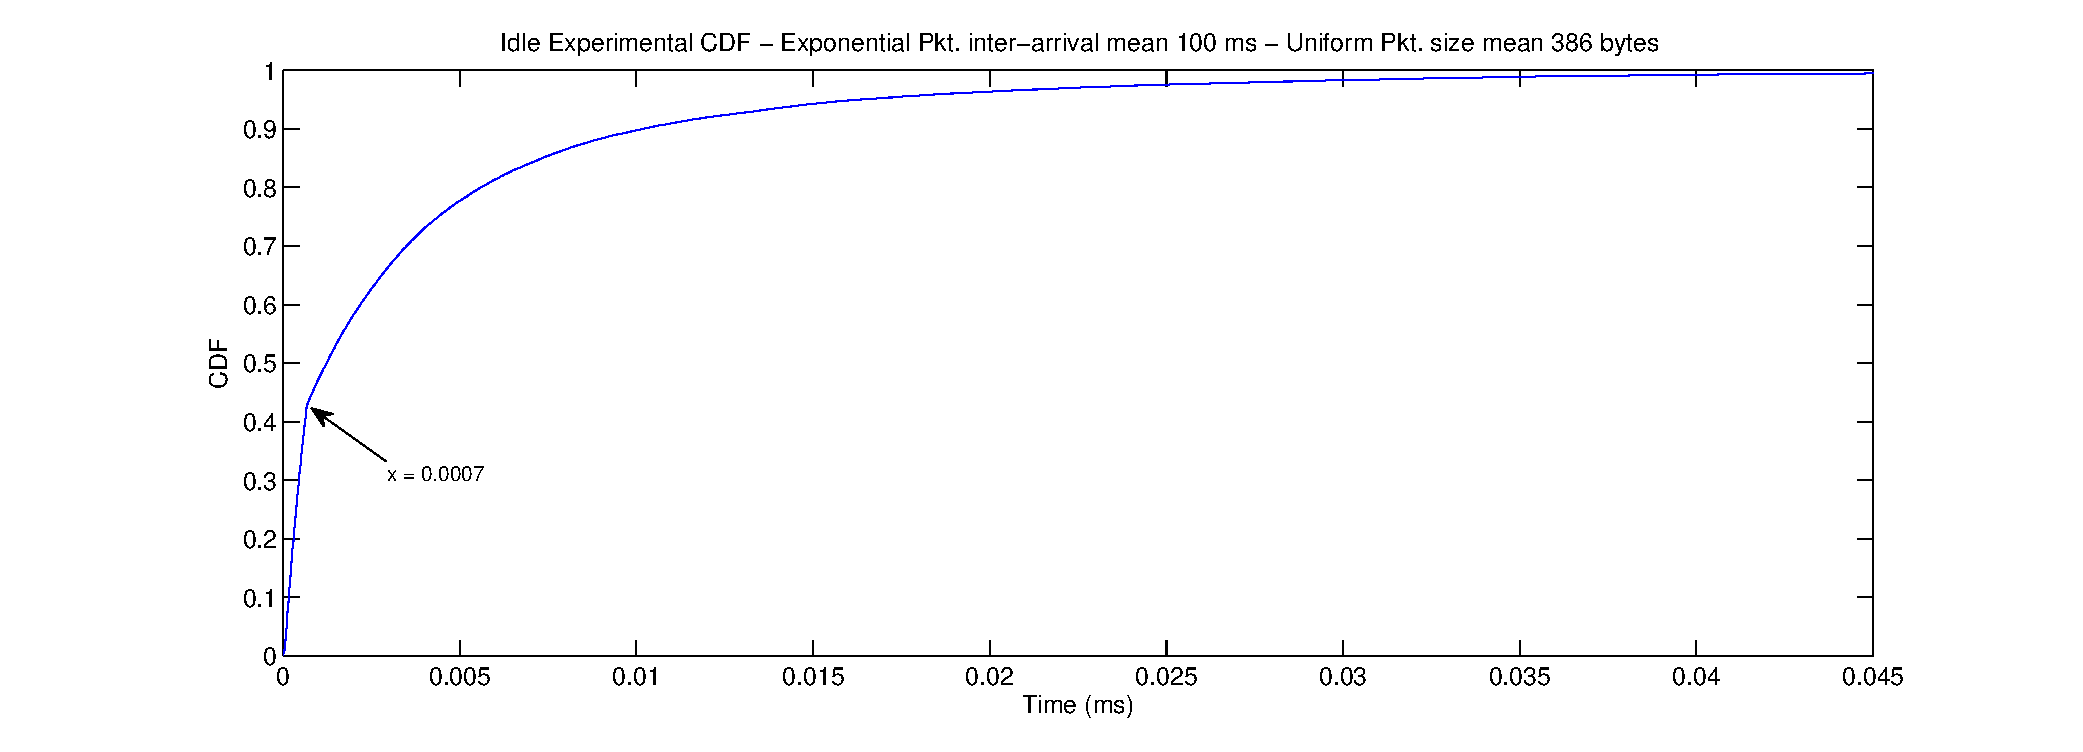
\includegraphics[width=\textwidth, trim = 0mm 0mm 0mm 0mm, clip]{images/results/GlobalView/cdf_globalview}
	\caption{Example of an Idle distribution using exponential interarrival time and constant packet size}
	\label{fig:cdf_globalview}
\end{figure}

The same behavior is observed for different distributions for the packet size and packet inter-arrival times.

\clearpage
\subsubsection{Idle Distribution Sensitivity}
In addition to the experiments developed to visually test the mixture idle distribution, we also tested the idle distribution sensitivity for different active distributions, meaning that, we test if the mixture idle distribution can still be used for different distributions for the packet sizes and inter-arrivals. Again, we generated a medium-load traffic using the traffic configuration presented in Table \ref{table:traffic_sensitivity} and the same user realization presented in Figure \ref{fig:test_model_network} and used different distributions for the packet size and packet inter-arrival times and compare the results.

The idle distribution is strongly affected by the packet inter-arrival times while the active distribution is determined by the packet sizes. We fixed one random distribution for the inter-arrival times while using different distributions with the same mean for the packet sizes. In Figure \ref{fig:cdf_composed} we present one example of these experiments. It can be observed that for the same type of distribution for the packet inter-arrival (idle) (i.e. Exponential inter-arrival with 100 ms of mean) and different distributions for the packet sizes (active), the idle periods distribution is almost insensitive to different active distributions.

\begin{figure}[h!]
	\centering
	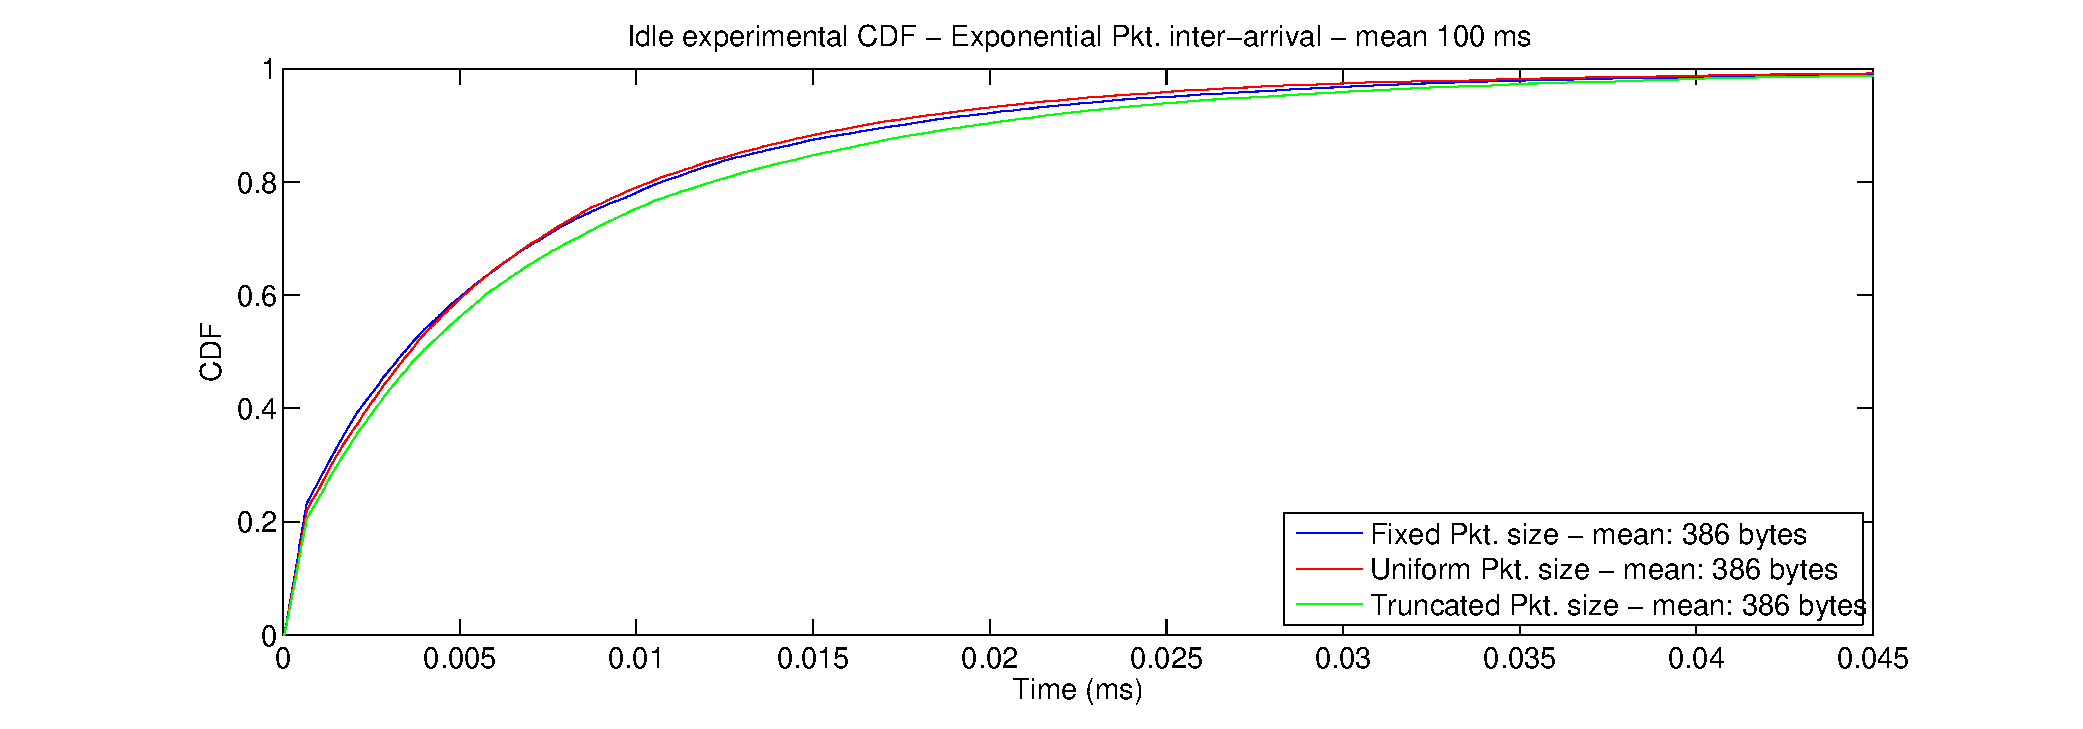
\includegraphics[width=\textwidth, trim = 0mm 0mm 0mm 0mm, clip]{images/results/GlobalView/cdf_pkt_sizes}
	\caption{Example of different Idle periods distribution for different distributions for the packet sizes. The active distribution do not affect the Idle function behavior.}
	\label{fig:cdf_composed}
\end{figure}

On the other hand, if the same tests are repeated fixing the distribution for the packet sizes and using different random distributions for the inter-arrival times, it can be observed how different random distributions affect the behavior of the idle function. This is represented in Figure \ref{fig:cdf_idle_compare}.

\begin{figure}[h!]
	\centering
	\subfloat[Different mean values for the same packet inter-arrival distribution affect the Idle distribution.]{
		\label{fig:cdf_exponential}
		\includegraphics[width=\textwidth, trim = 0mm 0mm 0mm 0mm, clip]{images/results/GlobalView/cdf_exponential}
	}
	\\
	\subfloat[Different packet inter-arrival distributions with same mean do not affect the final Idle periods distribution.]{
		\label{fig:cdf_idle_same_mean}
		\includegraphics[width=\textwidth, trim = 0mm 0mm 0mm 0mm, clip]{images/results/GlobalView/cdf_idle_same_mean}
	}
	\caption{Examples of different Idle functions for different Idle distributions}
	\label{fig:cdf_idle_compare}
\end{figure}

In Figure \ref{fig:cdf_exponential} a uniform distribution for the packet size with mean 386 bytes (256 - 512 bytes) has been used for all the tests while we used an exponential distribution with different mean values for the inter-arrival packet time. It can be observed how the proportionality between the mean values of the idle distribution increase/decrease the idle periods distribution represented in the \acs{CDF}. A low mean value for the packet inter-arrival means shorter idle times and, in extension, higher load in the network, making the packet inter-arrival dominant and reason of this behavior.

In Figure \ref{fig:cdf_idle_same_mean} is represented a experiment with an uniform distribution for the packet size with mean 386 bytes and different random distributions with the same mean for the inter-arrival times. It can be observed that the idle periods distribution is almost the same for different random distribution if they have the same mean.

Again, the same behavior is observed for different random distributions in the active and idle distributions.